\nnarticleheader{Team $\#$14169 M3 Challenge Submission: Keep on Trucking}{Alexander Greer '20, Gary Gao '21, and Xiaolong Huang '21}

\begin{center}
\textit{This article is an excerpt from Haverford's submission to the 2020 MathWorks Math Modeling (M3) Challenge. Teams of students were tasked with finding mathematical solutions to a large-scale problem over the course of 14 hours. If you are a rising junior or senior interested in participating in next year's competition, contact Mr. Bridge.}
\end{center}

\noindent
\textbf{Executive Summary}

Humanity’s ever-increasing reliance on technology necessitates a strong focus on environmental conservation and clean energy to ensure a safe and prosperous future. One goal of this effort is the use of electric vehicles in place of typical fossil fuel-based transportation. Diesel-powered semi-trucks account for a uniform 12\% of the transportation market, and so replacing these vehicles with electric counterparts would be an effective first step in the transition to wholly-electric transportation.

Here we present the answers to several logistical questions in the effort of switching the diesel semi-truck industry over to electric vehicles. One question is to determine how many electric semis will take over the trucking industry in the future. This is a question of when rather than if. Here, we make an informed prediction of this value based on data related to the current rate of production of semi-trucks throughout the country.

Another question is how to best position charging stations for electric semis along common trucking routes (or “corridors”). The optimal positioning of such stations is influenced by factors such as vehicle range and traffic flow. Here we present optimized charging locations along five standard corridors based on route length, battery capacity, and traffic information throughout each road.

A final question is to determine the prioritization of the development of the above electric stations. While electric vehicles will provide long-term benefits to our society, there may be short term consequences that result from infrastructure changes. Here we outline a prioritization order for the same five routes based on multiple economic and social factors such as political and economic support, as well as route length and associated traffic volume.

The conclusions outlined above and described more thoroughly throughout this work serve to incite the development of electric vehicle implementation. We hope that a broader understanding of the factors at play will lead to widespread adoption and the eventual universal acceptance of environmentally-conscious technologies.

\noindent
\textbf{Definitions}
\begin{itemize}
\item \noindent Commercial Battery Electric Vehicle (\textbf{CBEV} or \textbf{BEV})\\
\indent The above acronym will be used interchangeably to refer to electric semis.

\item \noindent Short Haul (\textbf{SH}), Regional Haul (\textbf{RH}), and Long Haul (\textbf{LH})\\
\indent The abbreviated forms of these vehicle types will be used for the sake of brevity.
\end{itemize}

\noindent
\textbf{Restatement of Problem \#2: "In It for the Long Haul"}

In this problem, we intend to determine the number of necessary CBEV charging stations for each of the five routes provided by the problem (San Antonio, TX to New Orleans, LA; Minneapolis, MN to Chicago, IL; Boston, MA to Harrisburg, PA; Jacksonville, FL to Washington, DC; Los Angeles, CA to San Francisco, CA). Additionally, we will determine the quantity of individual chargers necessary at each station. 

\noindent
\textbf{Assumptions}

\begin{assumption}
Multiple routes can be taken between two cities. Here we assume that drivers will always take the shortest route.

Justification – Drivers always seek to optimize their driven performance, which primarily involves fuel/energy efficiency. Therefore, we assume drivers will select the shortest route in order to expend the least amount of fuel/energy.
\end{assumption}

\begin{assumption}
Secondly, we assume that the drivers will have an 80\% charged battery at the start of their trip, and the driver will try to charge their truck whenever the battery is below 20\%.

Justification – Battery is optimally charged from 20 to 80 percent. The drivers and corporations will seek efficiency to maximize profit, so they will always charge their batteries in this way.
\end{assumption}

\begin{assumption}
Thirdly, we assume that there are a sufficient amount of charging stations around the city, and the charging stations on the highway are left to be built.

Justification – Cities are far more developed than highway resting stops and negates the need for developing new charging stations. In contrast, highway resting stops are spread far apart and are less incentivized.
\end{assumption}

\begin{assumption}
We assume that the traffic flow for semi trucks is constant throughout the day.

Justification – There is a large enough quantity of traffic flowing through the specified routes in order to assume a constant flow.
\end{assumption}

\begin{assumption}
Additionally, we assume that a CBEV battery has a 550 kWh capacity, and the distance to travel when fully charged is 250 miles.

Justification – These numbers fall within the average range and were the most common we found online, thus we used them in our calculations.
\end{assumption}

\noindent
\textbf{Data}
\begin{center}
	\begin{tabular}{|c|c|c|}
		\hline
		\textbf{Truck} & \textbf{Battery Size} & \textbf{Distance to Travel}\\
		\hline
		Freightliner eCascadia & 550 kWh & 250 miles\\
		\hline
		Chanje V8100 & 150 kWh & 150 miles\\
		\hline
		Tesla Semi Truck & Approximately 600 kWh & 300 miles\\
		\hline
	\end{tabular}
\end{center}
\medskip
\begin{center}
	\begin{tabular}{|c|c|}
		\hline \textbf{Routes} & \textbf{Distance}\\
		\hline San Antonio, TX to/from New Orleans, LA & 543 miles\\
		\hline Minneapolis, MN to/from Chicago, IL & 408 miles\\
		\hline Boston, MA to/from Harrisburg, PA & 390 miles\\
		\hline Jacksonville, FL to/from Washington, DC & 706 miles\\
		\hline Los Angeles, CA to/from San Francisco, CA & 382 miles\\
		\hline
	\end{tabular}
\end{center}

\renewcommand{\thefigure}{1}
\begin{figure}[h]
  \begin{center}
    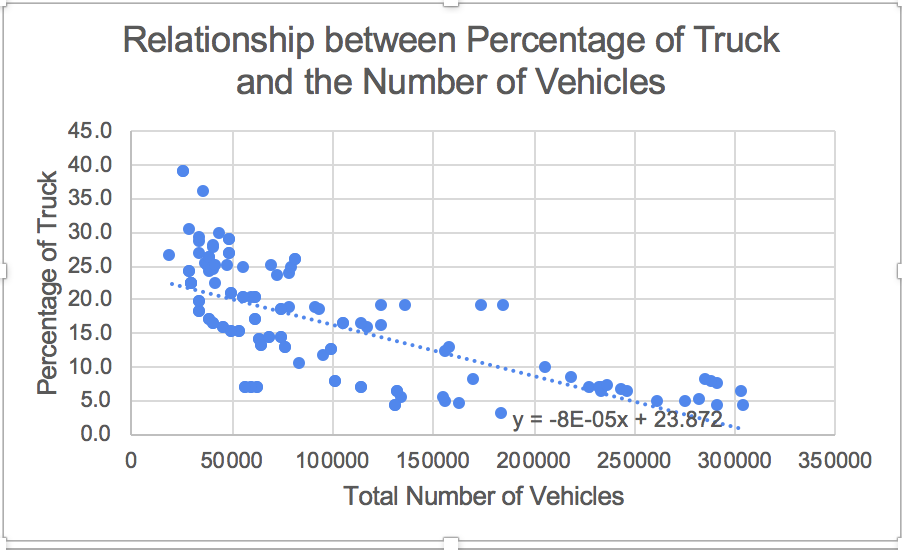
\includegraphics[scale=.95]{M3_image}
  \end{center}
  \caption{Corridor Data, MathWorks Math Modeling Challenge 2020, https://m3challenge.siam.org/node/478}
  \label{fig:1}
\end{figure}

\noindent
\textbf{Analysis}

We define distance to be D miles, charging speed to be C kW, battery size to be B kWh, distance that a truck can drive to be K miles, Price of each charger to be P dollars, average amount of semi trucks that passes through a certain point every day to be A trucks/day, the number of charging stations to be R, and the number of chargers at each station to be S.

We first look at the average amount of class 8 trucks here. From Corridor Data, MathWorks Math Modeling Challenge 2020, url, we can obtain the amount of total vehicles at a certain and the number of trucks at the certain point of the given route. However, the data of numbers of trucks are missing at certain points of the table. In order to obtain the missing data, we can take the average of the ratio between the number of trucks and the number of total vehicles to approximate the number of trucks when given the number of total vehicles.

We define the number of trucks to be B. We notice that the number of trucks is not equivalent to the number of class 8 trucks, so we can approximate the number of class 8 trucks by comparing the total number of trucks to the total number of semi trucks. We know that the number of semi trucks is 2 million and the total number of trucks is 15.5 million. Hence, we can approximate the number of semi trucks at a given point on the highway by: 
\[A = \frac{2}{15.5}\cdot B\]
\indent However, if we look at the graph of all available traffic data of percentages of Truck and total number of vehicles, we can see that the percentage of trucks when there are fewer vehicles is significantly higher than that when there are more vehicles, which suggests that the number of trucks tend to remain the same. Hence, we apply a linear regression on this set of data and add that function to our model. We define the number of vehicles to be E, which is as below:
\[A = \frac{2}{15.5}\cdot B = \frac{2}{15.5}\cdot(-8\cdot10^{-5}\cdot E+23.872)\cdot E\]
\indent We now have the number of trucks at a certain location. We then try to determine how many stations are needed for a route. Considering the cost, we will try to find the minimum charging stations that can fulfill the need. We know that, optimally, the truck is going to use 60\% of its battery, which is derived from our assumption that the truck is going to start at 80\% battery and charge whenever the battery gets below 20\%. Hence, we have the model: 
\[R = \frac{D}{\displaystyle \frac{3}{5}\cdot K}\]
\indent We now obtain models that can calculate the number of stations for a given route, and now we need to find out how many chargers are necessary for each station. We first need to determine how long it takes for a truck to charge. The time, which is defined as T, is equal to 60\% of the battery size (since we are only charging from 20\% to 80\%) divided by the charging speed, which is:
\[T = \frac{3B}{5C}\]
\indent We know that there are 24 hours in a day, and the number of trucks is the truck that passes through the place in that 24 hours. We also know from the last consumption that the traffic flow is constant. Hence, we have:
\[S = \frac{T}{24}\cdot A\]
\indent Now we have the general functions and we need to calculate the number of stations and the number of chargers at each station for each route. 

\noindent
\textbf{San Antonio, TX to/from New Orleans, LA:}

We try to find the number of stations by inserting the equation $\displaystyle R = \frac{D}{\frac{3}{5}\cdot K}$. We know that $D = 543$ miles, $K = 250$ miles. Inserting the constant, we have:
\[R = \frac{550}{150} \approx 4\]

We then try to find the number of chargers at each station:
\begin{align*}
	S &= \frac{T}{24}\cdot A\\
	&= \frac{T}{24}\cdot \frac{2}{15.5}\cdot(-8\cdot10^{-5}\cdot E+23.872)\cdot \frac{E}{100}\\
	&= \frac{1.33}{24}\cdot \frac{2}{15.5}\cdot(-8\cdot10^{-5}\cdot 77580+23.872)\cdot \frac{77580}{100}\\
	&\approx 108
\end{align*}
T
herefore, for each charging station we need 108 chargers. 

\noindent
\textbf{Minneapolis, MN to/from Chicago, IL:}

Similarly, we have
\[R = \frac{408}{150} \approx 3\]

Then,
\begin{align*}
	S &= \frac{T}{24}\cdot \frac{2}{15.5}\cdot(-8\cdot10^{-5}\cdot E+23.872)\cdot \frac{E}{100}\\
	&= \frac{1.33}{24}\cdot \frac{2}{15.5}\cdot(-8\cdot10^{-5}\cdot 103062+23.872)\cdot \frac{103062}{100}\\
	&\approx 115
\end{align*}

Therefore, we need 3 charging stations and for each charging station we need 115 chargers. 

\noindent
\textbf{Boston, MA to/from Harrisburg, PA:}

Similarly, we have
\[R = \frac{390}{150} \approx 3\]

Then,
\begin{align*}
	S &= \frac{T}{24}\cdot \frac{2}{15.5}\cdot(-8\cdot10^{-5}\cdot E+23.872)\cdot \frac{E}{100}\\
	&= \frac{1.33}{24}\cdot \frac{2}{15.5}\cdot(-8\cdot10^{-5}\cdot 75435+23.872)\cdot \frac{75435}{100}\\
	&\approx 96
\end{align*}

Therefore, we need 3 charging stations and for each charging station we need 96 chargers.

\noindent
\textbf{Jacksonville, FL to/from Washington, DC:}

Similarly, we have
\[R = \frac{709}{150} \approx 5\]

Then,
\begin{align*}
	S &= \frac{T}{24}\cdot \frac{2}{15.5}\cdot(-8\cdot10^{-5}\cdot E+23.872)\cdot \frac{E}{100}\\
	&= \frac{1.33}{24}\cdot \frac{2}{15.5}\cdot(-8\cdot10^{-5}\cdot 83803+23.872)\cdot \frac{83803}{100}\\
	&\approx 103
\end{align*}

Therefore, we need 5 charging stations and for each charging station we need 103 chargers.

\noindent
\textbf{Los Angeles, CA to/from San Francisco, CA:}

Similarly, we have
\[R = \frac{382}{150} \approx 3\]

Then,
\begin{align*}
	S &= \frac{T}{24}\cdot \frac{2}{15.5}\cdot(-8\cdot10^{-5}\cdot E+23.872)\cdot \frac{E}{100}\\
	&= \frac{1.33}{24}\cdot \frac{2}{15.5}\cdot(-8\cdot10^{-5}\cdot 134347+23.872)\cdot \frac{134347}{100}\\
	&\approx 126
\end{align*}

Therefore, we need 3 charging stations and for each charging station we need 126 chargers.

\noindent
\textbf{Conclusion}

Now we have tested all the routes and obtained valid solutions. Below is a list of the number of chargers necessary to supply each of the routes provided. 

\begin{center}
	\begin{tabular}{|c|c|}
		\hline \textbf{Routes} & \textbf{Number of Chargers}\\
		\hline San Antonio, TX to/from New Orleans, LA & 108 chargers\\
		\hline Minneapolis, MN to/from Chicago, IL & 115 chargers\\
		\hline Boston, MA to/from Harrisburg, PA & 96 chargers\\
		\hline Jacksonville, FL to/from Washington, DC & 103 chargers\\
		\hline Los Angeles, CA to/from San Francisco, CA & 126 chargers\\
		\hline
	\end{tabular}
\end{center}

\vspace{1.25cm}

\begin{center}
\textit{For more information on\\
the MathWorks Math Modeling Challenge,\\
including winning entries from\\
this year's competition,\\
visit https://m3challenge.siam.org/}
\end{center}
